In this chapter, applications of the proposed methods in simulating the quasi-2D systems are presented.
We first present the applications in simulating the SPC/E bulk water systems with up to $10^6$ atoms, and then report a spontaneous symmetry breaking phenomenon in negatively confined charged systems for the first time.

\section{All-atom SPC/E water systems}

In this section we perform all-atom MD simulations of SPC/E bulk water systems~\cite{berendsen1987missing} confined by two slabs with and without dielectric jumps utilizing the RBE2D method introduced in Chapter~\ref{chp_rbe2d}.
The parameter settings follow the same settings as in Section~\ref{sec::numerical}.

\subsection{SPC/E bulk water system without dielectric jumps}
\label{sec::waterhomo}

%To further demonstrate the accuracy and efficiency of the proposed RBE2D method, 
We perform MD simulations for the SPC/E bulk water system~\cite{berendsen1987missing}. 
The system has dimensions $L_x=L_y=H=55.9~\mathring{\text{A}}$ and consists of $17496$ atoms. 
Two purely repulsive shifted-truncated LJ walls (with $\varepsilon_{\text{atom-wall}}= k_{\text{B}}T)$ are located at $z=0$ and $z=H$.  
The simulations utilize a time step $\Delta t=1fs$, and $T$ is fixed at $298K$ by a NH thermostat with relaxation time $10fs$. 
Equilibration proceeds for $10^5$ time steps, followed by a $10^6$ steps production period, with configurations sampled every $100$ time steps. 
The cutoff is set as $r_c=10\mathring{A}$, and the ratio $L_z/H$ is fixed as $3$ to ensure that both the ELC and remainder error term are negligible.

\begin{figure}[ht!]
\centering
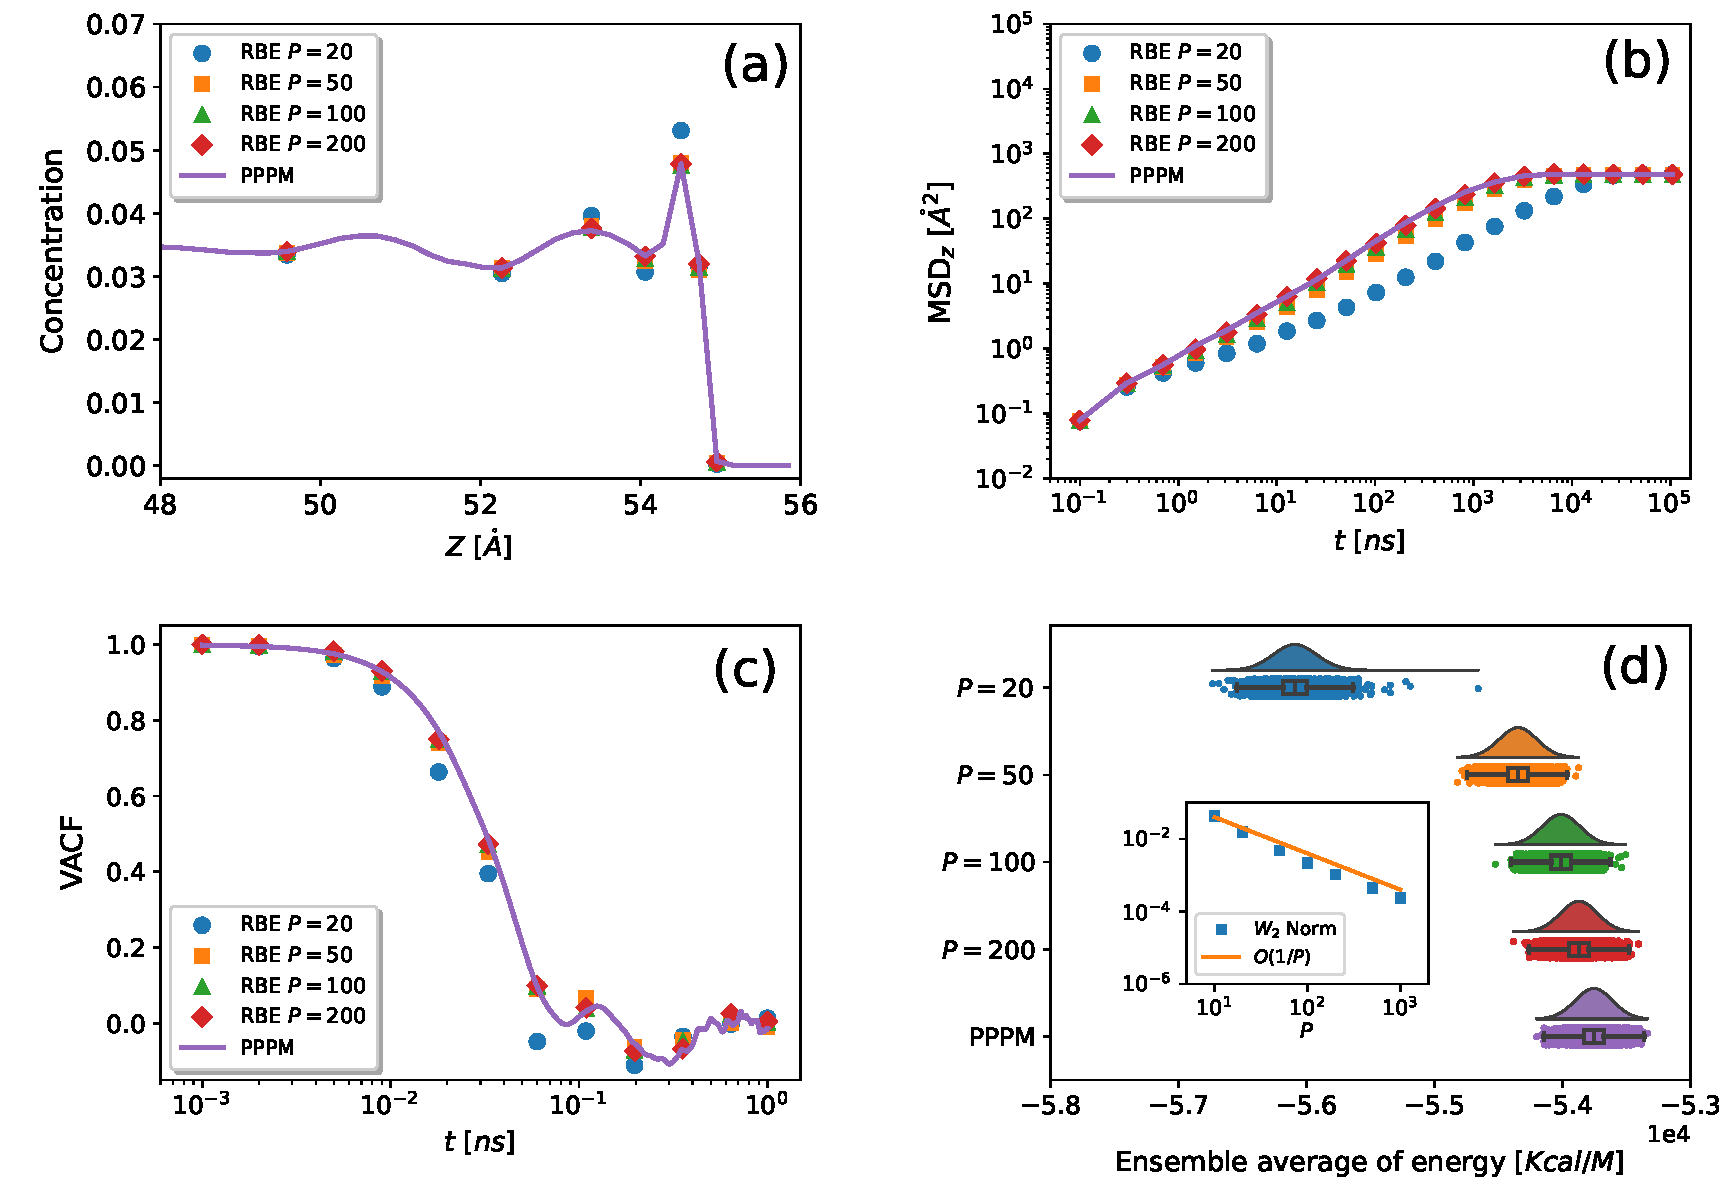
\includegraphics[width=1.0\linewidth]{figs/Density_new.pdf}
	\caption{MD results for a SPC/E bulk water system. (a)  Concentration of oxygen near the top surface; (b)  MSD along $z$-direction; (c)  VACF; and (d)  raincloud plots of the ensemble average distribution of the potential energy as well as a boxplot and raw data-points. The RBE2D with different batch sizes $P$ and the PPPM are plotted. The inset in (d) shows the convergence on the $W_2$ norm with $\mathcal{O}(1/P)$ rate.}
	\label{fig:Water}
\end{figure}

We analyze various equilibrium and dynamic properties of the system, including the oxygen concentration, the MSD in $z$, the VACF, and the distribution of potential energy $U$.
The results are summarized in Fig.~\ref{fig:Water}(a-d).
Notably, the RBE2D method yields highly consistent results in comparison to the PPPM method across all examined properties when $P \geq 100$. 
This underscores the RBE2D's ability to effectively capture spatiotemporal information across multiple scales in molecular dynamics simulations.

\subsection{Dielectrically confined SPC/E water}

%To further assess the comparison of both the accuracy and efficiency between the RBE2D and ICM-PPPM methods, 
We conclude the numerical tests with simulations of dielectrically confined SPC/E bulk water, and cross compare the RBE2D and ICM-PPPM methods. 
%The equilibrium temperature is set to $T=298K$. 
%The equilibration process was carried out for $50 ns$, followed by MD simulations on the NVT ensemble of $100ns$ for data collecting. 
One can refer to Sec.~\ref{sec::waterhomo} for most of the system setups.
Here the dielectric mismatches are introduced, set as $\gamma_{\text{top}}=\gamma_{\text{bot}}=-0.5$. 
The parameters of the ICM-PPPM method were automatically chosen~\cite{kolafa1992cutoff} to achieve a relative error of $\Delta=10^{-4}$, and the real space cutoff distance $r_c$ was set to $12\mathring{A}$, which was selected to optimize the performance of the ICM-PPPM method. 

\begin{figure}[ht]
\centering
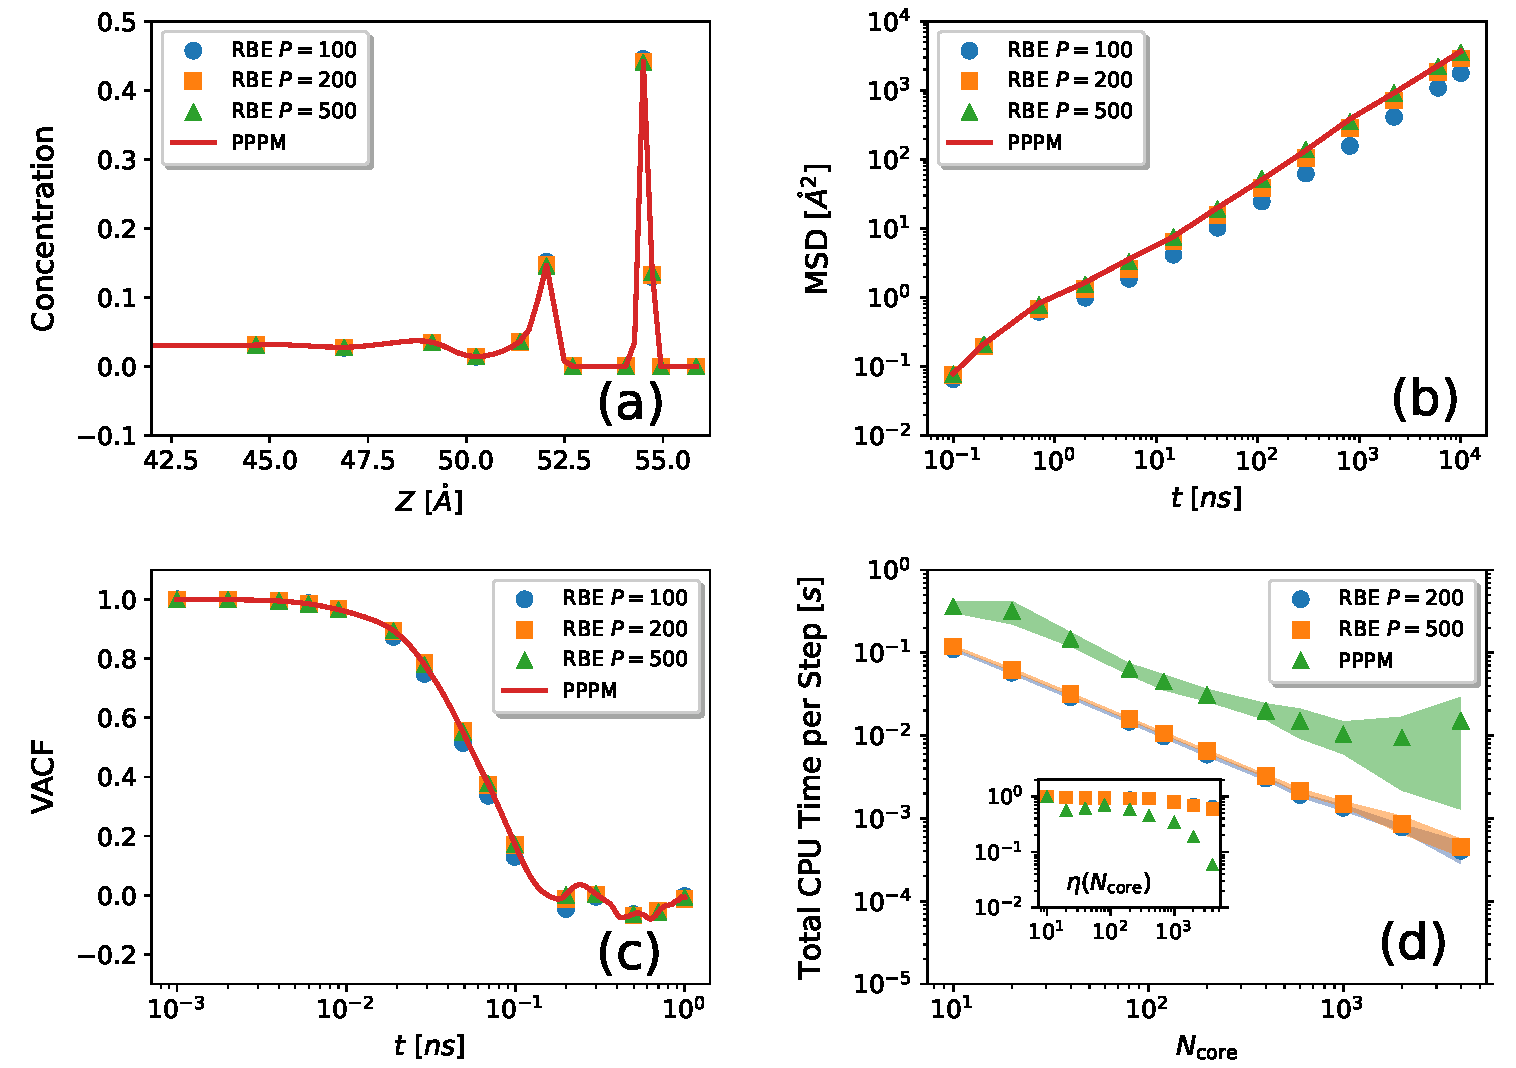
\includegraphics[width=1.0\linewidth]{figs/Dielectric.pdf}
    \caption{Distribution of oxygen atom {s} in SPC/E bulk water system (a), the MSD (b), the VACF (c), and comparison of time performance between RBE2D (with different $P$) and ICM-PPPM (d) are studied. 
    The inset in (d) shows  {the} corresponding strong parallel efficiency $\eta(N_{\text{core}})$ defined as Eq.~\eqref{eq::etau}. 
    The results derived from the RBE2D   {are} almost identical to those from the ICM-PPPM. 
     {The RBE2D based MD is about $1.5$ orders of magnitudes faster than the ICM-PPPM-based MD.}
    }
    \label{fig:den2}
\end{figure}

We first examine the concentration of oxygen along  {the} $z$-axis for a system comprising $53367$ atoms, the results are displayed in Fig.~\ref{fig:den2}(a). 
We again find  excellent agreement between the RBE2D and the ICM-PPPM when $P\geq 200$, whereas some small discrepancy is observed if one chooses $P=100$. 
The MSD and VACF are also calculated and shown in Figs.~\ref{fig:den2}(b-c).
The results clearly indicate that for dynamic properties of the water molecules (such as MSD and VACF), the results obtained by RBE2D is consistent   {with} that of the ICM-PPPM  {across} multiple time scales ($fs$ to $ns$). 

Finally, the CPU time and scalability data of both the RBE2D and ICM-PPPM methods are documented in Fig.~\ref{fig:den2}(d), based on simulating a water system containing $139968$ atoms. It is observed that, the RBE2D is more than 10 times faster than the ICM-PPPM method. 
Furthermore, the   {parallel efficiency} is shown in the inset of Fig.~\ref{fig:den2}(d), which indicates that RBE2D can remain a strong scaling of $60\%$ for up to $4000$ CPU cores, while that of ICM-PPPM drops to only about $5\%$, again demonstrating the strong   {parallel efficiency} of RBE2D method.  {We also provide a more detailed comparison between the RBE2D and ICM-PPPM methods in Fig.~\ref{fig:timedie} in the SM, using the same number of CPU cores (\( N_{\text{core}} = 64 \) and 1024) and a batch size of \( P = 200 \), with varying particle number $N$. 
The results clearly demonstrate that the RBE2D outperforms the ICM-PPPM across the range of \( N \) up to \( 10^6 \).}

\section{Broken symmetry in quasi-2D Coulomb systems}\label{sec::ssb}

% \subsection{Theoretical origin for oscillations}

% Eq.~\eqref{eq:G_point_charge} shows that the Green's function can be represented as a Sommerfeld integral, and the analytical form of $g(k, z, z_s)$ indicates that it has non-trival behaviors.
% Clearly, $g(k, z, z_s)$ is divergent at $k=k_0$ (given in Eq.~\eqref{eq:k0}), and as $\gamma_1\gamma_2$ increases to be larger than 1, $k_0$ will shift onto the positive real axis, then the Sommerfeld integral needs to be renormalized.
% Notice that when~$k \to k_0$, the divergent factor has the property
% \begin{equation}
%     \frac{1}{\gamma_1 \gamma_2 \exp{(-2 k L_z)} - 1} \to \frac{1}{2 L_z (k_0 - k)}\;,
% \end{equation}
% so that~$k_0$ is a first-order pole and the Cauchy principal value exists.
% Then Eq.~\eqref{eq:G_point_charge} for~$\gamma_1 \gamma_2 > 1$ cases is given by
% \begin{equation}\label{eq:G_pv}
%     G(\V{r}, \V{s}) = - \text{p.v.} \left[ \int_{0}^{+\infty} 2 g(k, z, z_s) J_0(k \Delta \rho) k \text{d}k \right]  \;,
% \end{equation}
% which can be calculated numerically. In what follows, we analyze the oscillatory behavior~(for more details, see Supplementary Information (SI)~\cite{SI}). First, the Green's function consists of integrals of the following general form
% \begin{equation}
%     I_o = \int_0^{\infty} \frac{J_0(k \D \rho) \text{e}^{-ka}}{\exp{\left( 2 L_z (k_0 - k) \right)} - 1} \text{d}k\;,
% \end{equation}
% where~$\D \rho$,~$k_0$ and~$a$ are all positive constants.
% We find that~$I_o$ can be further expanded as
% \begin{equation}
%     I_{o} = \frac{e^{-k_0 a}}{2L_z} \int_0^{\infty} \frac{J_0(k^\prime)}{k_0 \D \rho - k^\prime} \text{d}k^\prime + f(k_0, \D \rho, a),
% \end{equation}
% where~$k^\prime = k \D \rho$, and~$f(k_0, \D \rho, a)$ is a non-oscillatory analytic function which has minor contribution to~$I_o$.
% The first integral term can be understood as a function of~$k_0 \D \rho$, or denoted as~$I_{m} (k_0 \D \rho)$. Clearly, $I_{m}$ is solely controlled by~$k_0$, given different parameters of $\gamma$ and $L_z$.
% It is found that the first-order pole in $I_{m}$ provides the oscillatory mode, and we also numerical validated that the wavelength of the oscillation in $I_{m}$ indeed satisfies Eq.~\eqref{eq:wavelength}, which explains our findings.

\subsection{Spontaneous symmetry breaking in confined Coulomb systems}

To investigate the influence of dielectric nanoconfinement on the collective behavior of quasi-2D charged systems, we further developed a collection of numerical techniques to efficiently evaluate the Green's function Eq.~\eqref{eq:G_point_charge}. A novel Ewald-splitting type strategy is proposed, together with renormalization techniques and fast convergent quadrature schemes. All fine details and numerical validations are provided in the SI~\cite{SI}.
Our study focuses on a prototypical quasi-2D charged system, consisting of a binary mixture of charged particles described by the primitive model.
The system comprises~$N/2$ cations and~$N/2$ anions, each with the same diameter~$\tau_0$ and valence~$\pm 1$, resulting in an overall charge-neutral system. 
The Hamiltonian of the system is defined as follows, where~$i$ represents the~$i$-th particle with charge~$q_i$ located at position~$\V{r_i}$:
\begin{equation}
   \mathcal H = \frac{1}{2} \sum_{i,j=1}^{N}{}^\prime q_i q_j \ell_B G(\V r_i, \V r_j) + U_{\mathrm{LJ}}\;,\label{eq:Hamiltonian}
\end{equation}
The sum notation~$\sum_{i,j}{}^\prime$ implies that when~$i=j$, the function~$G(\V r, \V r)$ corresponds to the self-interaction term, and~$U_{\mathrm{LJ}}$ is the shift-truncated Lennard-Jones (LJ) potential energy used to model excluded-volume interactions. 
While this model disregards other important interactions observed in experimental realizations, it enables us to isolate the dielectric confinement effect. 
Similar systems have been studied recently in Refs.~\cite{dos2017simulations,liang2020harmonic,yuan2021particle}.

% two choices, 4 graphs or 3 graphs

\begin{figure}
	\centering
	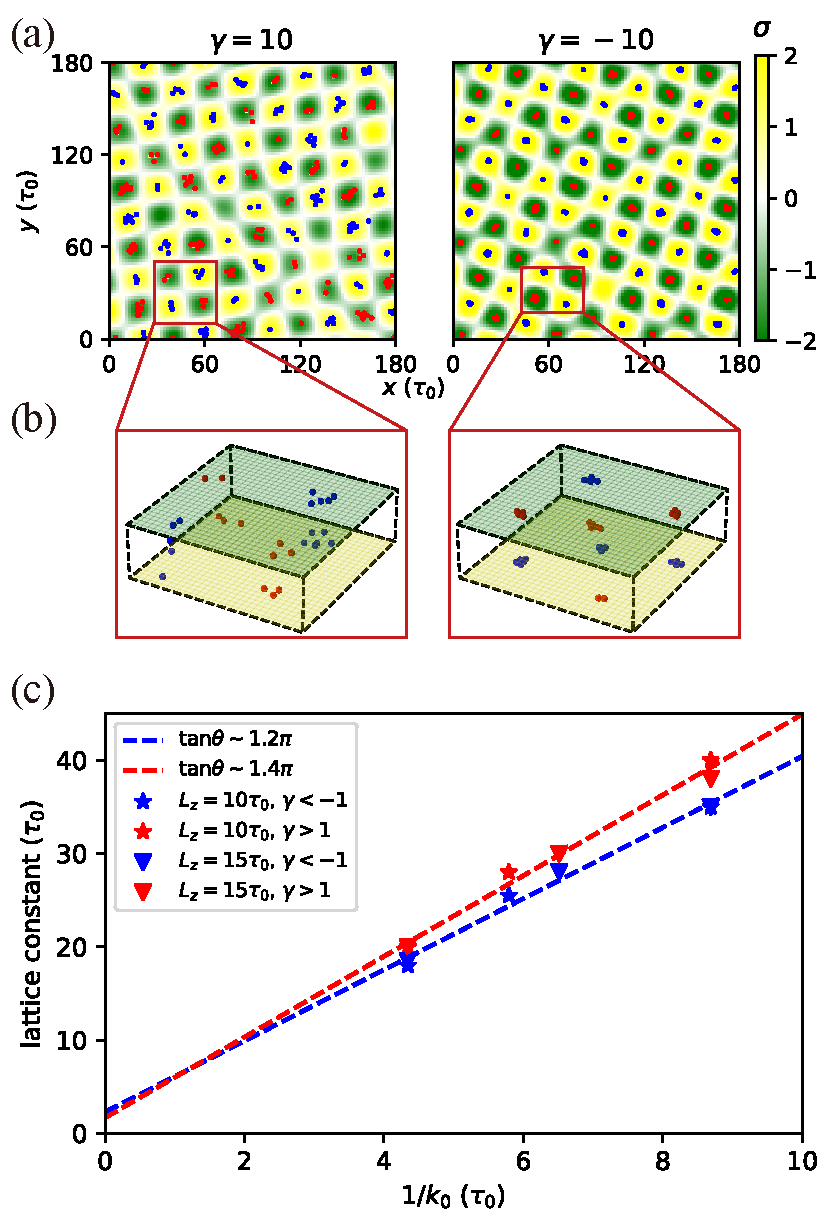
\includegraphics[width=1\textwidth]{figs/fig4.pdf}
	\caption{\label{fig:MD} 
        (a): Global particle distributions near the lower substrate and induced surface charge densities for~$\gamma = \pm 10$ and~$L_z = 10$. 
        Positive/negative induced surface charges are in yellow/green, while positive/negative particles are in red/blue, respectively.
        $\sigma$ unit:~$e_0/\tau_0^2$.
        (b): local 3D structures of the charged particles, enlarged from (a), while upper/lower boundaries are in green/yellow, respectively.
        (c): numerical validations for the relationship between the lattice constant and $k_0$. Symbols showing data points from individual simulations, dashed lines depict the linear fitted result.}
\end{figure}

In all the MD simulations, we maintain a constant box size in the~$xy$ plane of~$180\tau_0 \times 180\tau_0$, which is confirmed to eliminate boundary effects.
We vary the values of~$L_z$ and~$\gamma$ to adjust the wave number~$k_0$. 
The system contains~$300$ cations and~$300$ anions.
To isolate electrostatic effect, the reduced temperature $T_r$ is defined as~$T_r =k_{\mathrm B}T/\varepsilon_{\mathrm{Coul}}$, where~$\varepsilon_{\mathrm{Coul}} = e_0^2/(4 \pi \eps (3.5 \tau_0))$ and we set~$\varepsilon_{\mathrm{LJ}} = k_B T$ for both particle-particle and particle-substrate interactions. 
We integrate the temporal evolution using the Velocity-Verlet algorithm and control the temperature using the Anderson thermostat with stochastic collision frequency~$\omega = 0.1$ and reduced temperature~$T_r = 1$.

In the $\abs{\gamma}\leq 1$ regime, extensive simulation works have been done recently~\cite{liang2020harmonic,yuan2021particle} and no SSB phenomenon has been found, i.e., the density distributions of cations $\rho_{+}(\V r)$ and anions $\rho_{-}(\V r)$  always maintain symmetries of the system, given by 1) \emph{cross symmetry} in the confined space: $\rho_{+}(\V r)=\rho_{-}(\V r)$, 2) \emph{longitudinal symmetry}: $\rho_{\pm}(x,y,z)=\rho_{\pm}(x,y,L_z-z)$, and 3) \emph{transverse symmetry}: $\rho_{\pm}(x,y,z)=\rho_{\pm}(x',y',z)$. 
Our simulations give symmetric results for  $\abs{\gamma}\leq 1$, consistent as previous investigations (details are documented in SI~\cite{SI}). 
In the following discussions we will focus on the strongly polarizable cases of $\abs{\gamma}>1$, where SSB phenomena arise.

Fig.~\ref{fig:MD}(a) shows two snapshots for particle distributions near the lower substrate and the corresponding induced surface charge densities, for $\gamma=\pm10$ and $L_z=10$. It clearly shows, for the first time, SSB phenomena in such dielectric confined charged system: both the cross and transverse symmetries are broken when $\gamma=10$; and the remaining longitudinal symmetry is further broken when $\gamma=-10$ (as shown in Fig.~\ref{fig:MD}(b)).

Globally, we observe charged particles spontaneously forming square lattice structures near the substrates for both~$\gamma > 1$ and~$\gamma < -1$ cases, which breaks the transverse symmetry. 
We attribute this to the long-range single particle oscillatory field in the $xy$-plane, which directs particles self-organizing into a \emph{checkerboard} structure, so as to enhance the overall induced charge landscape, which helps confining particles in local potential wells.
Locally within each lattice site, two different particle structures are observed: for~$\gamma >1$, interfacial liquid phase is formed, while for~$\gamma < -1$, likely-charged particles self-assemble into 2D clusters, both can be understood by the near field behaviors due to a single confined particle, as was discussed and illustrated in Fig.~\ref{fig:force_x} (a).

Interestingly, in the longitudinal direction, we find that the interfacial liquids/clusters on opposing substrates are strongly correlated, i.e., there is a one-to-one “pairing” between the opposing particle structures, as show in Fig.~\ref{fig:MD}(b).
For $\gamma=10$, the longitudinal pairing is between symmetrically charged particles; while for $\gamma=-10$, the pairing becomes anti-symmetric, which further breaks the longitudinal symmetry. The symmetric/anti-symmetric longitudinal paring is due to the induced charge landscape on opposing substrates, it is clearly that for $\gamma=10$, the checkerboard structures would be matched symmetrically, while for $\gamma=-10$ a negative sign is added to the reflection rates, forming anti-symmetric pairs.

Finally, it is worth noting that the formed square lattices can be well-controlled via the single parameter~$k_0$, consistent with our theoretical prediction.
As shown in Figure \ref{fig:MD}(c), the lattice constant of the system is found to be proportional to $k_0^{-1}$, with various choice of $L_z$ and $\gamma$. 
Two slightly different linear relationships are observed, with fitted ratio~$1.2 \pi$ and~$1.4 \pi$ for~$\gamma < -1$ and~$\gamma > 1$ cases, respectively. 
The distance between neighboring clusters is found to be consistent with the second zero point of the induced surface charge density profile due to a single point charge (see subplots of Fig.~\ref{fig:force_x} (a)). The mechanism allows one to efficiently modulate the collective phase of dielectric confined systems.